\documentclass{beamer}
\usepackage[brazil]{babel}
\usepackage[utf8x]{inputenc} 
\PrerenderUnicode{ç}
\setbeamercovered{transparent=5}
\usetheme{Copenhagen}
\title{Physimulation: Biblioteca Gráfica para Simulações de Física}
\author{Alberto Hideki Ueda e Rafael Issao Miyagawa\\ \url{rafaelim@ime.usp.br} \url{alberto@ime.usp.br}}

\institute{Instituto de Matemática e Estatística\\Universidade de São Paulo}

\begin{document}

\frame{\titlepage}
\frame{\tableofcontents}
\section{Introdução}
\begin{frame}
  \frametitle{Motivação}
  \begin{itemize}
    \item "Por que temos disciplinas como física e estatística?" \\ 
      \
    \item Como relacionar com a computação e com os computeiros
      \
  \end{itemize} 
\end{frame}
\begin{frame}
  \frametitle{Objetivo}
  \begin{itemize}
    \item Criar um simulador físico para aulas de física \\
      \
    \item Problemas e soluções para simulações de ambientes físicos \\
      \
  \end{itemize}
\end{frame}
\section{Ferramentas e Conceitos}
\begin{frame}
  \frametitle{Linguagem e Plataformas}
  \begin{figure}
    
\includegraphics[scale=0.2]{ruby.jpg}
    \hspace{0.5cm}
    
\includegraphics[scale=0.4]{chipmunk.jpg}
    \hspace{0.5cm}
    
\includegraphics[scale=0.3]{gosu.jpg}
  \end{figure}
  \begin{block}{Ruby}
    Linguagem dinâmica e orientada a objetos
  \end{block}
  \begin{block}{Chipmunk}
    Biblioteca física voltada para jogos
  \end{block}
  \begin{block}{Gosu}
    Toolkit para criar interfaces de jogos
  \end{block}
\end{frame}
\begin{frame}
  \frametitle{Conceitos gerais}
  \begin{block}{Tempo de simulação}
    \begin{itemize}
      \item Fixo
      \item Variável
    \end{itemize}
  \end{block}
  \begin{block}{Broad Phase}
    \begin{itemize}
      \item Sweep and Prune, AABB tree e Spatial Hashing
    \end{itemize}
  \end{block}
  \begin{block}{Detecção de colisão (Narrow Phase)}
    \begin{itemize}
      \item Separating Axis Theorem
    \end{itemize}
  \end{block}
  \begin{figure}
    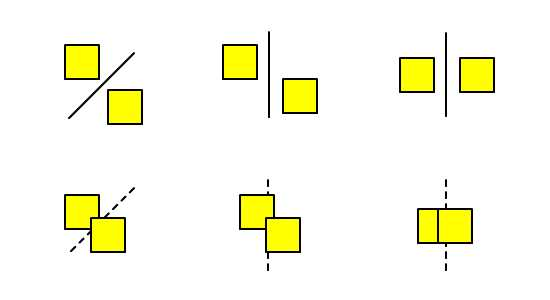
\includegraphics[scale=0.2]{SAT.jpg}
  \end{figure}
\end{frame}
\section{Resultados e Demonstrações} 

\begin{frame}
  \frametitle{Physimulation}
  \begin{itemize}
    \item Demonstrações 
  \end{itemize} 
\end{frame}

\section{Conclusão}
\begin{frame}
  \frametitle{github}
  \begin{figure}
    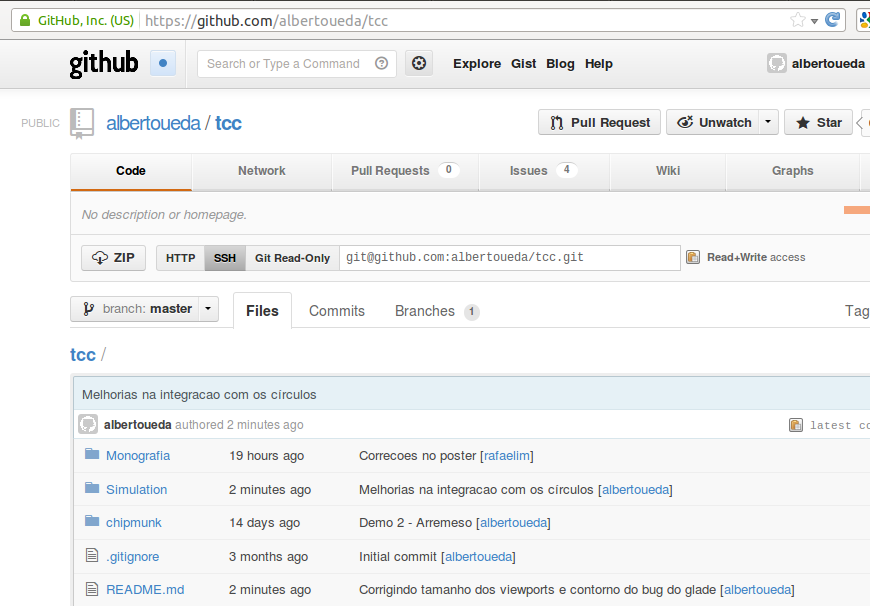
\includegraphics[scale=0.3]{github.png}
  \end{figure}
\end{frame}
\begin{frame}
  \frametitle{Próximos passos}
  \begin{itemize}
    \item Integração com Exercícios Programas da Poli/IME
    \item Mais primitivas. Ex: Molas e Pêndulos
    \item Migração do bind do ruby para versão do Chipmunk 6
  \end{itemize}
\end{frame}
\begin{frame}
  \frametitle{Agradecimentos}
  \begin{figure}
    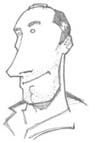
\includegraphics[scale=1]{coelhof.jpg}
  \end{figure}
  \begin{itemize}
    \item Prof. José Coelho
    \item João Pedro Kerr Catunda
  \end{itemize}
\end{frame}
\end{document}
